% =====================================================================
%  Introduction to Deep Learning — Class 19
%  Topic (course plan): Deep Networks
%  Subtopic (course plan): Regularization: Heuristic Methods, Early
%    stopping, Drop outs, Model averaging, Applying Noise
%  Sources (course plan): Prince Chapter 9, Bishop Chapter 9
%
%  Class 18 changed the objective and read off what the optimiser was
%  already doing.  This class changes the PROCEDURE and the DATA, and
%  leaves the objective alone.  Every method here is a heuristic, so
%  every claim is measured rather than asserted.
%
%  Order: stop the run, average many runs, average implicitly with
%  dropout, perturb the inputs, then borrow other data.
%
%  C variant: the B deck with the explicit filter form of the
%  early-stopping / weight-decay correspondence removed, since Bishop
%  (2024) states the correspondence but leaves the algebra to Exercise
%  9.6 and Bishop (1995a), and its ridge half was already removed from
%  the Class 18 C variant.  Bishop's qualitative statement stays.
%  See _shared/PLAN_Classes17_18_19.md.
%
%  Compile:  xelatex main.tex   (run twice)
% =====================================================================
\documentclass[aspectratio=169, 11pt]{beamer}

\usetheme{metropoliscustom}

\usepackage{graphicx}
\DeclareGraphicsExtensions{.pdf,.png,.jpg}
\graphicspath{{figs/}{Class19_Regularization_Heuristics/C_Textbook_Theorems_Only/figs/}}
\usepackage{amsmath, amssymb}
\usepackage{bm}
\usepackage{tikz}
\usetikzlibrary{arrows.meta, positioning, calc, decorations.pathreplacing,
                shapes.geometric, fit, backgrounds}
\tcbuselibrary{skins}

\definecolor{shc}{HTML}{341651}
\definecolor{tealc}{HTML}{1C7293}
\definecolor{dpc}{HTML}{800000}
\definecolor{accc}{HTML}{B8860B}

% ---- theorem environments -------------------------------------------
\setbeamertemplate{theorems}[numbered]
\usepackage{remreset}
\makeatletter\@removefromreset{theorem}{section}\makeatother
\renewcommand{\thetheorem}{\arabic{theorem}}
\newtheorem{lemmax}[theorem]{Lemma}
\newtheorem{propx}[theorem]{Proposition}
\newtheorem{corx}[theorem]{Corollary}
\newtheorem{defx}[theorem]{Definition}
\newtheorem{thmx}[theorem]{Theorem}

\newcommand{\bridge}[1]{%
  {\scriptsize\itshape\color{mcMuted} #1\par}\vspace{0.35em}}

\newcommand{\srcline}[1]{%
  \par\vspace{0.25em}%
  {\scriptsize\color{mcMuted}\hfill #1\par}}

\newcommand{\figsource}[1]{{\scriptsize\color{mcMuted} #1}}
\newcommand{\figcap}[2][0.90]{%
  \begin{center}\begin{minipage}{#1\textwidth}\centering
    {\scriptsize\color{mcMuted} #2}
  \end{minipage}\end{center}}

% =====================================================================
\title{Deep Networks}
\subtitle{Regularization: Heuristic Methods}
\author{Introduction to Deep Learning \ \textperiodcentered\ Class 19}
\institute{}
\date{}

\footleft{Introduction to Deep Learning}
\footright{Heuristic Regularization}
\titlelogos{}

\begin{document}

\maketitle

\begin{frame}{Outline}
  \tableofcontents
\end{frame}

% =====================================================================
\section{What Is Left to Change}
% =====================================================================

\begin{frame}{From the objective to the procedure}
  \bridge{Class 18 added a term to the objective and read off the
  preference the optimiser already had; neither touched the procedure or
  the data.}
  \vspace{0.05em}
  {\scriptsize
  \renewcommand{\arraystretch}{1.22}
  \begin{tabular}{@{}l@{\hspace{1.4em}}l@{\hspace{1.4em}}l@{}}
    \textbf{Where the bias goes} & \textbf{Mechanism} & \textbf{Class}\\
    the objective & $\lambda\|\mathbf{w}\|^2$, the lasso & 18\\
    the optimiser & step size, batch size & 18\\
    the architecture & sharing, residual paths & 18\\
    \textbf{the stopping rule} & \textbf{early stopping} & \textbf{today}\\
    \textbf{the number of runs} & \textbf{ensembles, dropout} & \textbf{today}\\
    \textbf{the data} & \textbf{noise, augmentation} & \textbf{today}\\
  \end{tabular}}
  \vspace{0.4em}

  \begin{redhighlight}
    Everything today is a heuristic: justified by measurement, not by a
    guarantee. So everything today is measured.
  \end{redhighlight}
\end{frame}

\begin{frame}{Notation for today}
  \vspace{0.4em}
  {\footnotesize
  \renewcommand{\arraystretch}{1.32}
  \begin{columns}[T, onlytextwidth]
    \begin{column}{0.49\textwidth}
      \begin{tabular}{@{}l@{\hspace{1.5em}}l@{}}
        $\tau$ & the iteration index\\
        $\eta$ & the step size, as in Class 13\\
        $\alpha$ & the weight-decay strength\\
        $\lambda_i$ & eigenvalues of $\mathbf{H}$, as in Class 13\\
      \end{tabular}
    \end{column}
    \begin{column}{0.49\textwidth}
      \begin{tabular}{@{}l@{\hspace{1.5em}}l@{}}
        $M$ & members of a committee\\
        $y_m(\mathbf{x})$ & the prediction of member $m$\\
        $\rho$ & the dropout probability\\
        $\sigma_x^2$ & variance of noise added to inputs\\
      \end{tabular}
    \end{column}
  \end{columns}}
  \vspace{0.6em}

  \begin{itemize}\itemsep0.26em
    \item Bishop writes the dropout \emph{keep} probability and Prince
          writes the \emph{drop} probability; the two are $1-\rho$ and
          $\rho$
    \item $h(\mathbf{x})$ is still the regression function of Class 17
  \end{itemize}
  \srcline{Bishop \& Bishop (2024), \S9.3.1, \S9.6; Prince (2023), \S9.3.}
\end{frame}

% =====================================================================
\section{Early Stopping}
% =====================================================================

\begin{frame}{The learning curve is a measurement, not a prediction}
  \begin{center}
    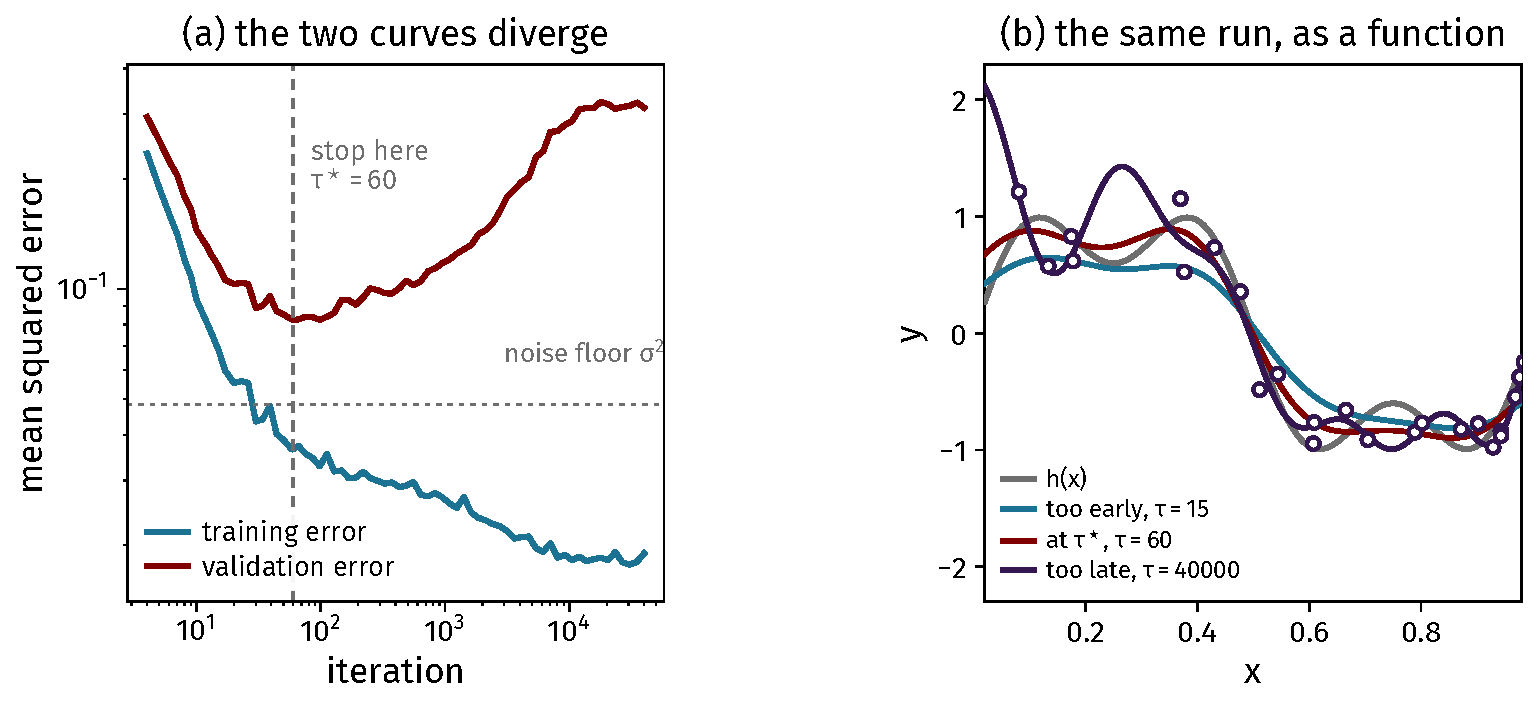
\includegraphics[width=0.665\linewidth]{learning_curves}
  \end{center}
  \figcap[0.97]{(a) training error falls throughout; validation error
  turns at $\tau^\star = 60$. (b) the fit before, at, and long after
  that point: the coarse shape arrives first, the noise afterwards.}
  \srcline{Bishop \& Bishop (2024), Fig.~9.7; Prince (2023), Fig.~9.6.}
\end{frame}

\begin{frame}{Stopping early, in practice}
  \vspace{0.15em}
  {\footnotesize
  \begin{itemize}\itemsep0.30em
    \item One hyperparameter: how many steps. Unlike every other
          hyperparameter, it does \alert{not} need repeated training
    \item Train once, evaluate on the validation set every $T$ steps,
          keep the parameters whenever the validation error improves,
          and return the best set at the end
    \item So the cost is one run plus the evaluations, against one run
          \emph{per value} for a penalty coefficient
    \item In the language of Class 17: increasing $\tau$ increases the
          effective model complexity, so stopping early moves back down
          the curve rather than changing the model
  \end{itemize}}
  \srcline{Prince (2023), \S9.3.1; Bishop \& Bishop (2024), \S9.3.1.}
\end{frame}

\begin{frame}{Stopping early is weight decay in disguise}
  \vspace{0.1em}
  \begin{propx}[Early stopping and weight decay]\label{th:early}
    \small
    For a quadratic error, gradient descent started from
    $\mathbf{w} = \mathbf{0}$ reaches the stiff eigen-directions of $\mathbf{H}$
    quickly and the flat ones slowly, so a run of $\tau$ steps has
    fitted the directions with large $\lambda_i$ and not yet reached
    those with small $\lambda_i$. That is the same selection a
    weight-decay penalty makes, and the correspondence is quantitative:
    the quantity $\eta\tau$ acts as the \alert{reciprocal} of the
    regularization coefficient.
  \end{propx}
  \vspace{0.35em}
  {\footnotesize
  \begin{itemize}\itemsep0.26em
    \item So training longer is regularising less, and the stopping
          iteration is a hyperparameter of exactly the same kind as
          $\lambda$
    \item Class 17's effective model complexity is the same idea again:
          it grows with $\tau$, and stopping early keeps it small
  \end{itemize}}
  \srcline{Bishop \& Bishop (2024), \S9.3.1, Fig.~9.8 and Exercise 9.6;
  Bishop (1995a).}
\end{frame}

\begin{frame}{Descent on a quadratic, drawn}
  \vspace{-0.3em}
  \begin{center}
    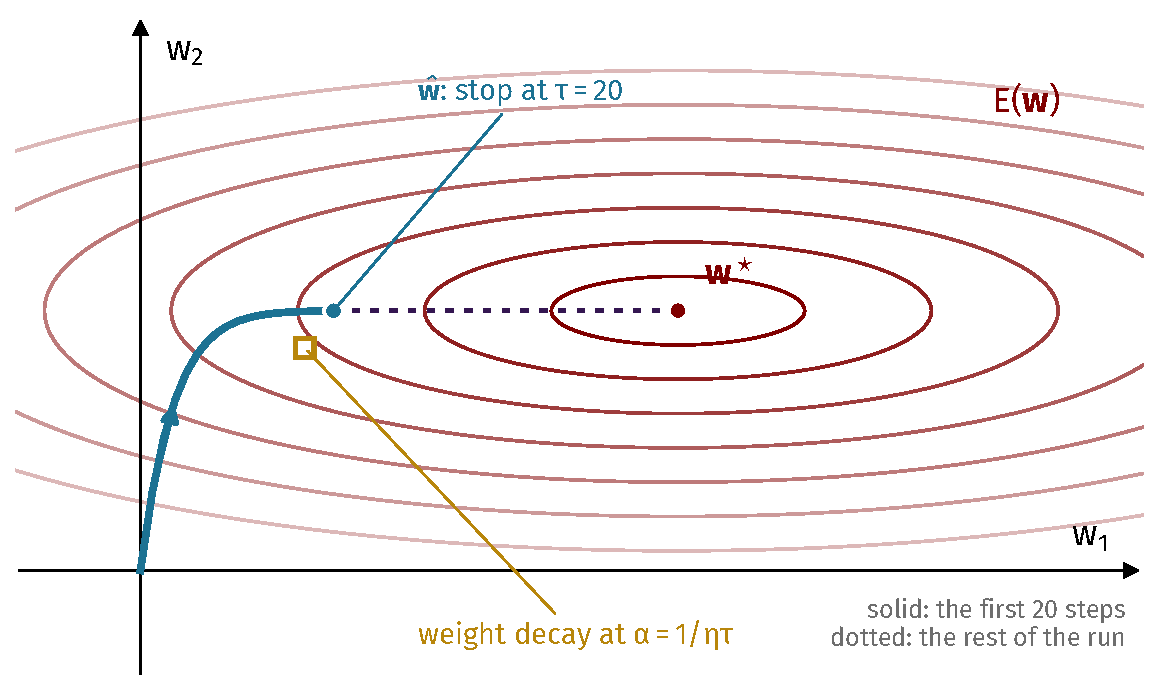
\includegraphics[width=0.66\linewidth]{early_stopping_path}
  \end{center}
  \vspace{-0.6em}
  {\tiny\color{mcMuted}
  Contours of the error, axes on the eigenvectors of the Hessian. From
  the origin, descent moves first along $w_2$, the stiff direction, and
  only later along $w_1$ towards $\mathbf{w}^\star$. Stopping at
  $\hat{\mathbf{w}}$ lands beside what a weight-decay penalty at
  $\alpha = 1/\eta\tau$ would have given.
  \hfill Bishop \& Bishop (2024), Fig.~9.8.\par}
\end{frame}

% =====================================================================
\section{Averaging Models}
% =====================================================================

\begin{frame}{Committees}
  \vspace{-0.2em}
  \[
    y_{\mathrm{COM}}(\mathbf{x}) = \frac{1}{M}\sum_{m=1}^{M} y_m(\mathbf{x}),
    \qquad
    p(y \mid \mathbf{x}) = \frac{1}{M}\sum_{m=1}^{M} p_m(y \mid \mathbf{x}) .
  \]
  \vspace{-0.5em}
  {\footnotesize
  \begin{itemize}\itemsep0.26em
    \item Rather than select the best of several models, keep all of
          them and average
    \item Class 17 showed why this should help: the \alert{variance}
          term is what differs between models fitted to different
          samples, and averaging cancels it
    \item The members must differ. Different initializations, different
          architectures, or --- most simply --- different data
    \item \alert{Bagging}: draw $N$ points from the training set
          \emph{with replacement}, $M$ times over, and fit one model to
          each resample
  \end{itemize}}
  \srcline{Bishop \& Bishop (2024), Eqs.~9.42--9.43; Breiman (1996);
  Prince (2023), \S9.3.2.}
\end{frame}

\begin{frame}{What averaging is worth}
  \vspace{-0.3em}
  \begin{thmx}[Committee error]\label{th:com}
    \small
    Write $y_m(\mathbf{x}) = h(\mathbf{x}) + \epsilon_m(\mathbf{x})$ and let
    $E_{\mathrm{AV}} = \frac{1}{M}\sum_m \mathbb{E}_{\mathbf{x}}[\epsilon_m^2]$.
    If the errors have zero mean and are uncorrelated,
    $\mathbb{E}_{\mathbf{x}}[\epsilon_m \epsilon_l] = 0$ for $m \neq l$, then
    \[
      E_{\mathrm{COM}} = \frac{1}{M}\, E_{\mathrm{AV}} .
    \]
    Without any assumption at all,
    $E_{\mathrm{COM}} \leq E_{\mathrm{AV}}$.
  \end{thmx}
  \vspace{0.2em}
  \begin{itemize}\itemsep0.24em
    \item The first statement is spectacular and its hypothesis is
          almost never true: members trained on resamples of one data
          set make \alert{correlated} errors
    \item The second needs nothing and is the one to rely on: averaging
          never hurts
  \end{itemize}
  \srcline{Bishop \& Bishop (2024), Eqs.~9.44--9.50 and Exercise 9.15.}
\end{frame}

\begin{frame}{Proof of both halves}
  \vspace{-0.25em}
  {\footnotesize
  \begin{itemize}\itemsep0.30em
    \item \focus{1}{By definition
          $E_{\mathrm{COM}} = \mathbb{E}_{\mathbf{x}}\big[(\tfrac1M\sum_m
          \epsilon_m)^2\big]$.}
    \item \focus{2}{Expanding the square gives
          $\tfrac{1}{M^2}\sum_m \mathbb{E}[\epsilon_m^2]
           + \tfrac{1}{M^2}\sum_{m \neq l} \mathbb{E}[\epsilon_m\epsilon_l]$.}
    \item \focus{3}{If the cross terms vanish, only the first sum
          survives: $\tfrac{1}{M^2}\cdot M E_{\mathrm{AV}}
          = E_{\mathrm{AV}}/M$. \hfill $\square$}
    \item \focus{4}{For the bound, apply Jensen's inequality to the
          convex function $t \mapsto t^2$:
          $(\tfrac1M\sum_m \epsilon_m)^2 \leq
          \tfrac1M\sum_m \epsilon_m^2$ pointwise in $\mathbf{x}$.}
    \item \focus{5}{Taking $\mathbb{E}_{\mathbf{x}}$ of both sides gives
          $E_{\mathrm{COM}} \leq E_{\mathrm{AV}}$, with no assumption on
          the correlations. \hfill $\square$}
  \end{itemize}}
  \vspace{-0.2em}
  \begin{redhighlight}
    The factor $M$ is a best case that requires independence. The
    inequality is free.
  \end{redhighlight}
\end{frame}

\begin{frame}{The promise, and what arrives}
  \begin{center}
    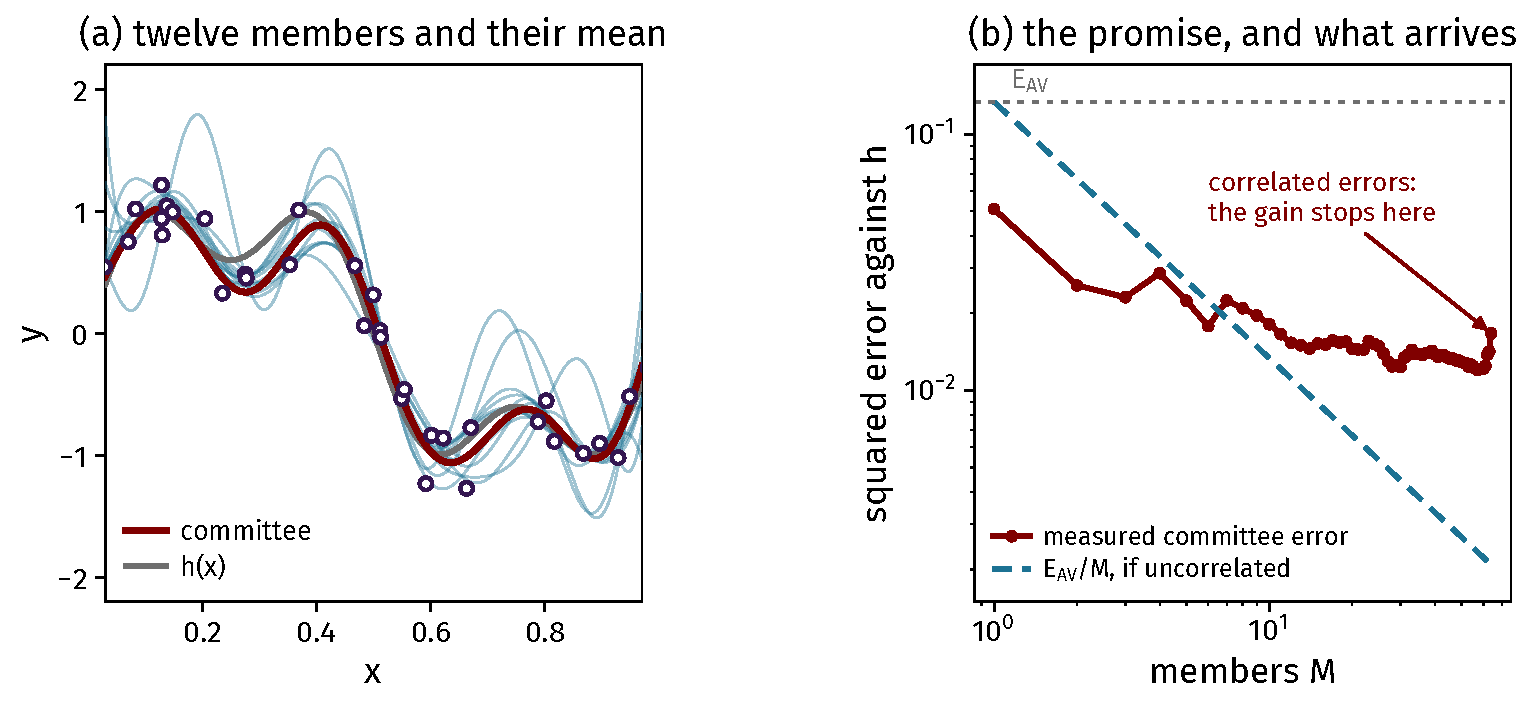
\includegraphics[width=0.70\linewidth]{ensemble_gain}
  \end{center}
  \figcap[0.97]{(a) twelve members fitted to bootstrap resamples, and
  their mean. (b) the committee error against $M$: it falls by about
  $4.5$ and flattens, where $1/M$ would promise $64$. The members'
  errors are correlated.}
\end{frame}

% =====================================================================
\section{Dropout}
% =====================================================================

\begin{frame}{An ensemble you do not have to train}
  \vspace{-0.3em}
  \begin{center}
  \begin{tikzpicture}[>=Stealth, font=\scriptsize, scale=0.86,
      nd/.style={circle, draw=shc, fill=shc!14, line width=0.9pt,
                 minimum size=0.40cm, inner sep=0pt},
      off/.style={circle, draw=mcMuted, fill=black!7, line width=0.7pt,
                  minimum size=0.40cm, inner sep=0pt},
      cn/.style={shc!55, line width=0.6pt},
      dim/.style={black!12, line width=0.6pt}]

    % ---------- full network -----------------------------------------
    \begin{scope}
      \node[nd] (a1) at (0,0.55) {};  \node[nd] (a2) at (0,-0.35) {};
      \node[nd] (b1) at (1.4,1.25) {}; \node[nd] (b2) at (1.4,0.45) {};
      \node[nd] (b3) at (1.4,-0.35) {}; \node[nd] (b4) at (1.4,-1.15) {};
      \node[nd] (c1) at (2.8,0.10) {};
      \foreach \i in {1,2} \foreach \j in {1,2,3,4} \draw[cn] (a\i)--(b\j);
      \foreach \j in {1,2,3,4} \draw[cn] (b\j)--(c1);
      \node[shc] at (1.4,-1.85) {full network};
    \end{scope}

    % ---------- thinned copy 1 ---------------------------------------
    \begin{scope}[shift={(4.9,0)}]
      \node[nd] (d1) at (0,0.55) {};  \node[nd] (d2) at (0,-0.35) {};
      \node[nd]  (e1) at (1.4,1.25) {}; \node[off] (e2) at (1.4,0.45) {};
      \node[nd]  (e3) at (1.4,-0.35) {}; \node[off] (e4) at (1.4,-1.15) {};
      \node[nd] (f1) at (2.8,0.10) {};
      \foreach \i in {1,2} \foreach \j in {1,3} \draw[cn] (d\i)--(e\j);
      \foreach \i in {1,2} \foreach \j in {2,4} \draw[dim] (d\i)--(e\j);
      \foreach \j in {1,3} \draw[cn] (e\j)--(f1);
      \foreach \j in {2,4} \draw[dim] (e\j)--(f1);
      \node[shc] at (1.4,-1.85) {one thinned copy};
    \end{scope}

    % ---------- thinned copy 2 ---------------------------------------
    \begin{scope}[shift={(9.8,0)}]
      \node[nd] (g1) at (0,0.55) {};  \node[nd] (g2) at (0,-0.35) {};
      \node[off] (h1) at (1.4,1.25) {}; \node[nd]  (h2) at (1.4,0.45) {};
      \node[off] (h3) at (1.4,-0.35) {}; \node[nd] (h4) at (1.4,-1.15) {};
      \node[nd] (k1) at (2.8,0.10) {};
      \foreach \i in {1,2} \foreach \j in {2,4} \draw[cn] (g\i)--(h\j);
      \foreach \i in {1,2} \foreach \j in {1,3} \draw[dim] (g\i)--(h\j);
      \foreach \j in {2,4} \draw[cn] (h\j)--(k1);
      \foreach \j in {1,3} \draw[dim] (h\j)--(k1);
      \node[shc] at (1.4,-1.85) {another};
    \end{scope}
  \end{tikzpicture}
  \end{center}
  \vspace{-0.15em}
  \begin{itemize}\itemsep0.24em
    \item At every step a fresh random mask deletes each non-output node
          with probability $\rho$, and the update is computed on what is
          left
    \item With $M$ non-output nodes there are $2^{M}$ thinned networks;
          almost none is ever visited twice, and they \alert{share} their
          weights
  \end{itemize}
  \srcline{Srivastava et al.\ (2014); Bishop \& Bishop (2024), \S9.6.1,
  Fig.~9.17; Prince (2023), Fig.~9.8.}
\end{frame}

\begin{frame}{How to predict with $2^M$ networks}
  \vspace{-0.2em}
  \begin{propx}[The weight-scaling inference rule]\label{th:wsr}
    \small
    A node kept with probability $1-\rho$ contributes, in expectation
    over masks, $(1-\rho)$ times what it contributes when always
    present. Multiplying its outgoing weights by $(1-\rho)$ at test time
    therefore matches the expected input to the next node, and lets one
    deterministic pass stand in for the average over masks.
  \end{propx}
  \vspace{0.1em}
  {\footnotesize
  \begin{itemize}\itemsep0.22em
    \item The exact rule would be
          $p(y\mid\mathbf{x}) = \sum_{\mathbf{R}} p(\mathbf{R})\,p(y\mid\mathbf{x},\mathbf{R})$,
          a sum over exponentially many masks
    \item \alert{Monte Carlo dropout} instead samples $10$ or $20$ masks
          and averages, which also gives a spread and so an uncertainty
    \item Typical rates: $\rho \approx 0.5$ for hidden nodes,
          $\rho \approx 0.2$ for inputs
  \end{itemize}}
  \srcline{Bishop \& Bishop (2024), Eq.~9.51; Prince (2023), \S9.3.3.}
\end{frame}

\begin{frame}{Dropout, measured}
  \begin{center}
    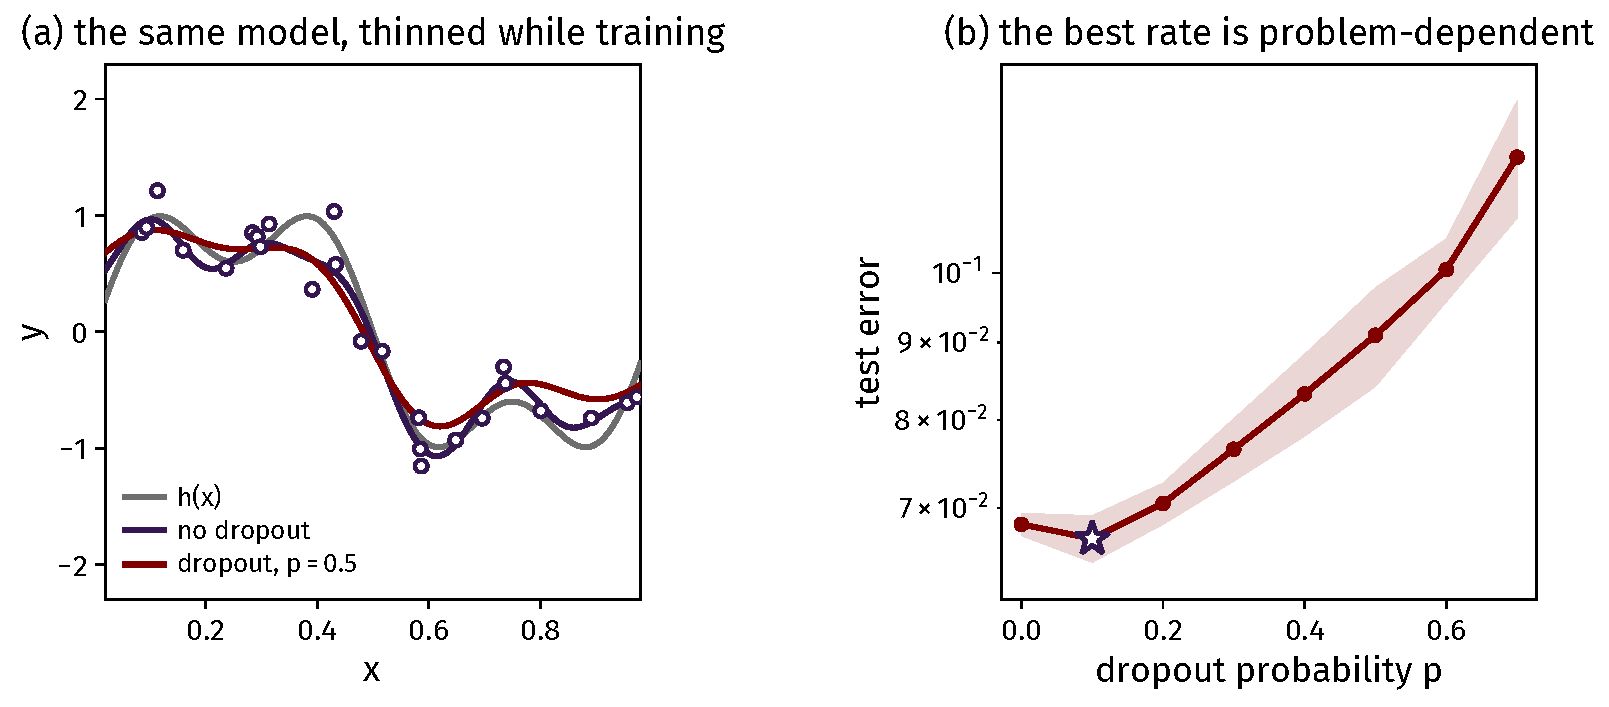
\includegraphics[width=0.70\linewidth]{dropout}
  \end{center}
  \figcap[0.97]{(a) the same model with and without dropout: the dropout
  fit is smoother where the data are thin. (b) test error against the
  rate, six runs each. The best rate here is $0.1$, not the usual
  $0.5$: with $44$ features there is little redundancy to spare.}
\end{frame}

\begin{frame}{Why removing a unit removes a kink}
  \vspace{0.15em}
  {\footnotesize
  \begin{itemize}\itemsep0.28em
    \item Suppose three units conspire: one raises the slope, the next
          lowers it, the third restores it. The net effect is a local
          wiggle between two training points
    \item That wiggle costs nothing on the training set, so no amount of
          further training removes it
    \item Delete one of the three --- which is what dropout does --- and
          the compensation fails, the output changes over a whole
          half-space, and the loss notices
    \item The next gradient step then repairs it, and over many steps
          the conspiracy is dismantled
  \end{itemize}}
  \vspace{0.1em}
  \begin{redhighlight}
    Dropout reaches structure that the loss alone cannot see, because it
    changes which parameters are asked to explain the data.
  \end{redhighlight}
  \srcline{Prince (2023), \S9.3.3 and Fig.~9.9.}
\end{frame}

% =====================================================================
\section{Applying Noise}
% =====================================================================

\begin{frame}{Noise on the inputs is a penalty}
  \vspace{-0.25em}
  \begin{thmx}[Input noise and weight decay]\label{th:noise}
    \small
    Let the model be linear, $\hat y = \mathbf{x}^{\mathsf T}\mathbf{w}$, and add
    noise $\bm{\epsilon}$ with mean $\mathbf{0}$ and covariance
    $\sigma_x^2 \mathbf{I}$ to every input. Then
    \[
      \mathbb{E}_{\bm{\epsilon}}\big[((\mathbf{x}+\bm{\epsilon})^{\mathsf T}\mathbf{w} - Y)^2\big]
      \;=\; (\mathbf{x}^{\mathsf T}\mathbf{w} - Y)^2 \;+\; \sigma_x^2 \|\mathbf{w}\|^2 ,
    \]
    so training on noisy inputs is exactly weight decay with
    $\lambda = \sigma_x^2$. For a nonlinear model the same expansion
    leaves a penalty on $\partial \hat y / \partial \mathbf{x}$ instead.
  \end{thmx}
  \vspace{0.05em}
  {\footnotesize
  \begin{itemize}\itemsep0.20em
    \item The proof is one line: expand the square and use
          $\mathbb{E}[\bm{\epsilon}] = \mathbf{0}$ and
          $\mathbb{E}[\bm{\epsilon}\bm{\epsilon}^{\mathsf T}] = \sigma_x^2\mathbf{I}$
    \item The nonlinear version penalises \alert{sensitivity of the
          output to the input}, which is what smoothness means
  \end{itemize}}
  \srcline{Bishop (1995b); Prince (2023), \S9.3.4.}
\end{frame}

\begin{frame}{The equivalence, checked}
  \begin{center}
    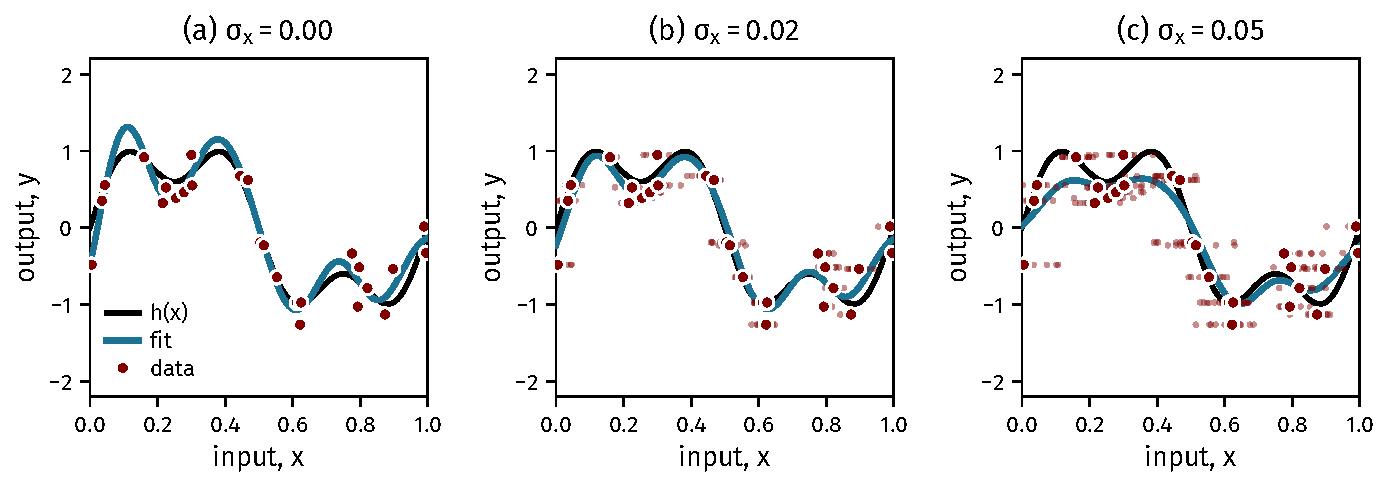
\includegraphics[width=0.94\linewidth]{input_noise}
  \end{center}
  \vspace{-0.7em}
  {\tiny\color{mcMuted}
  Noise of standard deviation $\sigma_x$ added to the batch inputs at
  every step of SGD, at three levels; the small dots are ten samples of
  the perturbed data. More noise gives a smoother fit. For a model
  linear in its inputs the equivalence is exact: trained with noise and
  solved with ridge at $\lambda = \sigma_x^2$, the weights differ by
  under $2\%$ at every level tried.
  \hfill Prince (2023), Fig.~9.10.\par}
\end{frame}

\begin{frame}{Three places to put noise}
  \vspace{0.1em}
  {\scriptsize
  \renewcommand{\arraystretch}{1.34}
  \begin{tabular}{@{}l@{\hspace{1.1em}}l@{\hspace{1.1em}}l@{}}
    \textbf{Noise on} & \textbf{Effect} & \textbf{Known as}\\
    the inputs & penalises $\partial\hat y/\partial\mathbf{x}$ & ---\\
    the inputs, worst case & robustness to the worst perturbation &
      adversarial training\\
    the weights & prefers wide flat minima & ---\\
    the labels & discourages certainty & label smoothing\\
    the activations & multiplicative Bernoulli noise & dropout\\
  \end{tabular}}
  \vspace{0.6em}

  {\footnotesize
  \begin{itemize}\itemsep0.24em
    \item Label smoothing assumes a fraction $\rho$ of the labels are
          wrong and belong equally to the other classes, which stops the
          pre-softmax activations running away
    \item Dropout is the same idea applied to activations, which is why
          it sits in this list as well as the previous section
  \end{itemize}}
  \srcline{Prince (2023), \S9.3.4.}
\end{frame}

% =====================================================================
\section{Borrowing Other Data}
% =====================================================================

\begin{frame}{When the data set is the constraint}
  \vspace{-0.25em}
  \begin{center}
  \begin{tikzpicture}[>=Stealth, font=\scriptsize, scale=0.86,
      bx/.style={rounded corners=2pt, draw, line width=1.0pt,
                 text width=2.55cm, minimum height=1.05cm,
                 align=center, inner sep=4pt},
      nt/.style={mcMuted, align=center, text width=3.1cm}]
    \node[bx, draw=shc,   fill=shc!10]   (a) at (0,0)
      {\textbf{transfer}\\ pre-train elsewhere,\\ refit the head};
    \node[bx, draw=tealc, fill=tealc!10] (b) at (3.9,0)
      {\textbf{multi-task}\\ one trunk,\\ several outputs};
    \node[bx, draw=dpc,   fill=dpc!10]   (c) at (7.8,0)
      {\textbf{self-supervised}\\ hide part of the input,\\ predict it};
    \node[bx, draw=accc,  fill=accc!12]  (d) at (11.7,0)
      {\textbf{augmentation}\\ transform the input,\\ keep the label};

    \node[nt, below=4pt of a] {needs a related\\ labelled set};
    \node[nt, below=4pt of b] {needs several\\ label types};
    \node[nt, below=4pt of c] {needs no\\ labels at all};
    \node[nt, below=4pt of d] {needs a known\\ invariance};
  \end{tikzpicture}
  \end{center}
  \vspace{0.1em}
  \begin{itemize}\itemsep0.24em
    \item All four are ways of getting more constraint per parameter
          without collecting more labelled examples of the actual task
    \item Augmentation is the invariance route of Class 18, taken
          through the data rather than the architecture
  \end{itemize}
  \srcline{Prince (2023), \S9.3.6--9.3.8; Bishop \& Bishop (2024), \S9.1.3.}
\end{frame}

\begin{frame}{The three routes, drawn}
  \begin{center}
    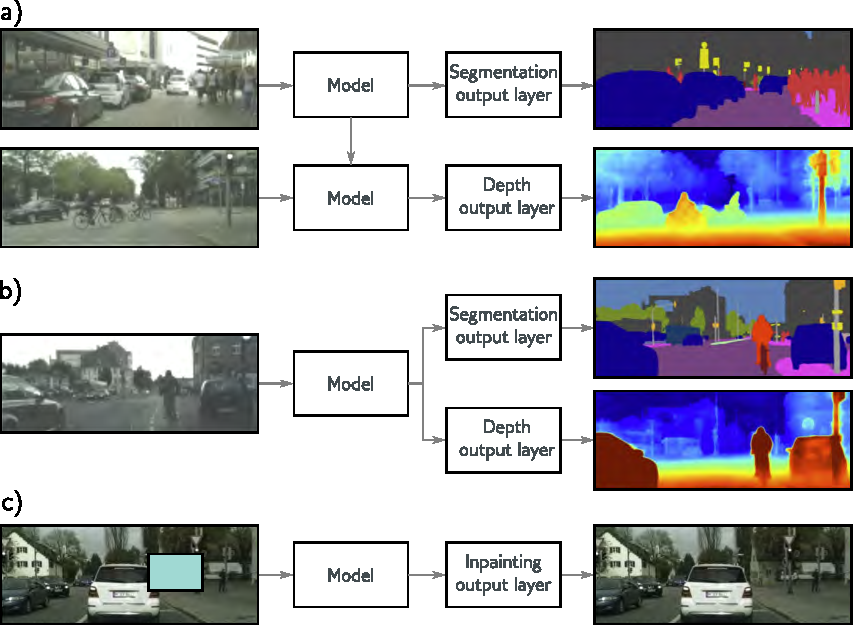
\includegraphics[height=0.505\textheight]{P_RegTransferMultiC}
  \end{center}
  \figcap[0.97]{(a) transfer learning: train on a secondary task with
  plentiful labels, then replace the head. (b) multi-task learning: one
  trunk, several outputs. (c) generative self-supervision: hide part of
  the input and train the network to restore it, so no labels are needed
  at all. Prince (2023), Fig.~9.12.}
\end{frame}

\begin{frame}{Augmentation}
  \vspace{-0.2em}
  \begin{center}
  \begin{tikzpicture}[font=\scriptsize, scale=0.92,
      im/.style={rounded corners=1.5pt, draw=shc, line width=0.9pt,
                 minimum width=1.55cm, minimum height=1.15cm,
                 fill=shc!8, align=center}]
    \node[im, fill=dpc!14, draw=dpc] (o) at (0,0) {original};
    \foreach \i/\lab in {1/{flip}, 2/{crop}, 3/{rotate},
                         4/{recolour}, 5/{blur}, 6/{noise}} {
      \node[im] at ({1.85*\i},0) {\lab};
    }
    \draw[decorate, decoration={brace, amplitude=5pt, mirror},
          mcMuted, line width=0.8pt]
      (-0.85,-0.78) -- (11.9,-0.78);
    \node[mcMuted] at (5.5,-1.35)
      {every one of these still has the same label};
  \end{tikzpicture}
  \end{center}
  \vspace{0.05em}
  {\footnotesize
  \begin{itemize}\itemsep0.24em
    \item Each transformation must be one the label is genuinely
          invariant to; a vertical flip is fine for a bird and wrong for
          a digit
    \item For text: substitute synonyms, or translate out and back.
          For audio: change the gain of frequency bands
    \item The model is being taught what to \alert{ignore}, which is a
          statement about the task and not about the data set
  \end{itemize}}
  \srcline{Prince (2023), \S9.3.8, Fig.~9.13; Bishop \& Bishop (2024),
  Fig.~9.1.}
\end{frame}

\begin{frame}{Augmentation, on an image}
  \begin{center}
    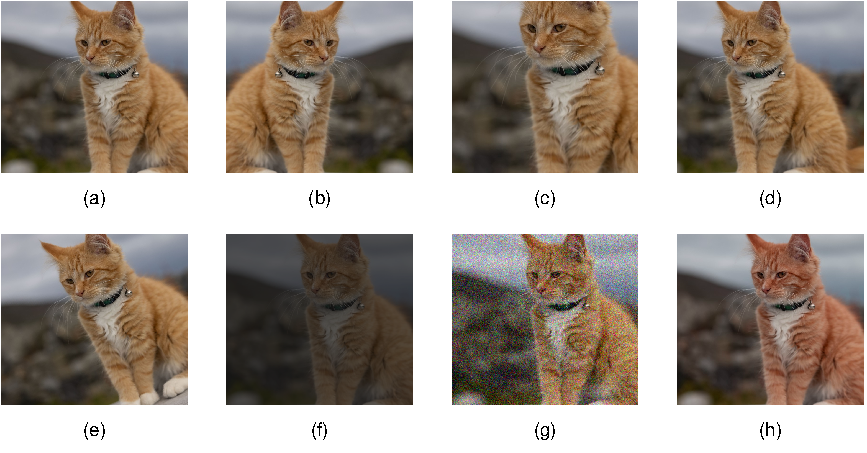
\includegraphics[height=0.50\textheight]{Bishop9_1}
  \end{center}
  \figcap[0.97]{(a) the original image, then (b) horizontal inversion,
  (c) scaling, (d) translation, (e) rotation, (f) brightness and
  contrast, (g) additive noise, (h) colour shift. Every one still has
  the same label. Bishop \& Bishop (2024), Fig.~9.1.}
\end{frame}

\begin{frame}{The Bayesian view: an infinite committee}
  \vspace{-0.5em}
  \begin{defx}[Bayesian prediction]\label{th:bayes}
    \small
    Instead of one parameter vector, keep a posterior over all of them,
    \[
      p(\mathbf{w} \mid \mathcal{D}) \propto
        \Big[\textstyle\prod_n p(Y_n \mid \mathbf{x}_n, \mathbf{w})\Big] p(\mathbf{w}),
      \qquad
      p(y \mid \mathbf{x}, \mathcal{D}) = \int p(y \mid \mathbf{x}, \mathbf{w})\,
        p(\mathbf{w} \mid \mathcal{D})\, \mathrm{d}\mathbf{w} .
    \]
  \end{defx}
  \vspace{0.1em}
  {\footnotesize
  \begin{itemize}\itemsep0.22em
    \item This is a committee with one member per parameter vector,
          weighted by how well it fits and how plausible it was
    \item Class 18's penalty was the same prior $p(\mathbf{w})$, used to pick
          the single most probable member instead of averaging
    \item For a network the integral is intractable, so every practical
          method approximates it --- and Monte Carlo dropout is one such
          approximation
  \end{itemize}}
  \srcline{Prince (2023), \S9.3.5, Eqs.~9.11--9.12.}
\end{frame}

\begin{frame}{The posterior, drawn}
  \vspace{-0.3em}
  \begin{center}
    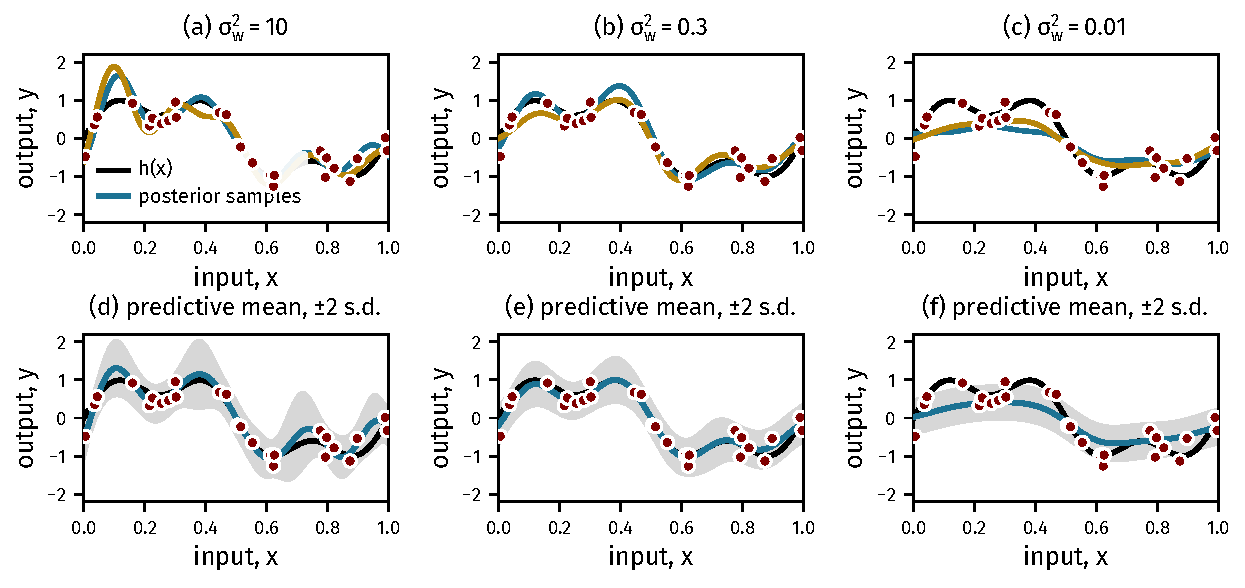
\includegraphics[width=0.84\linewidth]{bayesian}
  \end{center}
  \vspace{-0.75em}
  {\tiny\color{mcMuted}
  The bump model with a Gaussian prior, where the posterior is exact.
  (a--c) two parameter vectors drawn from it under priors of three
  variances: a tighter prior gives smaller parameters and smoother
  functions. (d--f) the average over all parameter vectors, with two
  standard deviations shaded: the band narrows from $1.08$ to $0.49$.
  \hfill Prince (2023), Fig.~9.11.\par}
\end{frame}

% =====================================================================
\section{Putting It Together}
% =====================================================================

\begin{frame}{The whole toolbox, across three classes}
  \vspace{-0.1em}
  {\scriptsize
  \renewcommand{\arraystretch}{1.20}
  \begin{tabular}{@{}l@{\hspace{0.9em}}l@{\hspace{0.9em}}l@{\hspace{0.9em}}l@{}}
    \textbf{Method} & \textbf{Acts on} & \textbf{Costs} & \textbf{Class}\\
    weight decay, lasso & the objective & one run per $\lambda$ & 18\\
    step size, batch size & the optimiser & nothing extra & 18\\
    sharing, residual paths & the architecture & must know the symmetry & 18\\
    early stopping & the stopping rule & one run, plus validation & 19\\
    ensembling, bagging & the number of models & $M$ trainings, $M$ inferences & 19\\
    dropout & the activations & slower convergence & 19\\
    input, weight, label noise & the data & one hyperparameter each & 19\\
    augmentation & the data & more compute per epoch & 19\\
    transfer, self-supervision & other data & a second training stage & 19\\
  \end{tabular}}
  \vspace{0.4em}

  \begin{redhighlight}
    Every row buys the same thing --- less variance --- and each pays in
    a different currency: compute, hyperparameters, or knowledge about
    the task.
  \end{redhighlight}
\end{frame}

\begin{frame}{Takeaways}
  \vspace{-0.15em}
  {\scriptsize
  \begin{enumerate}\itemsep0.24em
    \item Early stopping is the cheapest regularizer there is: one run,
          and the hyperparameter is read off a curve you were plotting
          anyway
    \item On a quadratic it selects the same directions weight decay
          would, with $\eta\tau$ acting as the reciprocal of the
          penalty coefficient (Proposition~\ref{th:early})
    \item Averaging $M$ models divides the error by $M$ only if their
          errors are uncorrelated; what always holds is
          $E_{\mathrm{COM}} \leq E_{\mathrm{AV}}$ (Theorem~\ref{th:com})
    \item In practice the members are correlated, and the measured gain
          was a factor of $4.5$ where $1/M$ promised $64$
    \item Dropout approximates an ensemble over $2^M$ weight-sharing
          networks; at test time one scaled pass stands in for it
          (Proposition~\ref{th:wsr})
    \item Noise on the inputs is weight decay exactly, for a linear
          model, and a penalty on $\partial\hat y/\partial\mathbf{x}$ in
          general (Theorem~\ref{th:noise})
    \item These are heuristics. Every one of the numbers above was
          measured on one small problem, and the defaults that circulate
          were calibrated on much larger ones
  \end{enumerate}}
  \bridge{Class 20 turns from how to train a network to what to build:
  the tutorials, and then convolutional networks.}
\end{frame}

\begin{frame}[allowframebreaks]{References}
  \vspace{0.3em}
  {\scriptsize
  \begin{enumerate}\itemsep0.30em
    \item C.\ M.\ Bishop \& H.\ Bishop, \emph{Deep Learning: Foundations
          and Concepts}, Springer, 2024. \S9.3.1 (Figs.~9.7--9.8);
          \S9.6 (Eqs.~9.42--9.51, Fig.~9.17); Exercises 9.6, 9.14, 9.15.
    \item S.\ J.\ D.\ Prince, \emph{Understanding Deep Learning}, MIT
          Press, 2023. \S9.3 (Eqs.~9.11--9.12, Figs.~9.5--9.13).
    \item C.\ M.\ Bishop, ``Regularization and complexity control in
          feed-forward networks'', ICANN 1995.
    \item C.\ M.\ Bishop, ``Training with noise is equivalent to
          Tikhonov regularization'', \emph{Neural Computation} 7(1),
          1995.
    \item L.\ Breiman, ``Bagging predictors'', \emph{Machine Learning}
          24(2), 1996.
    \item N.\ Srivastava, G.\ Hinton, A.\ Krizhevsky, I.\ Sutskever \&
          R.\ Salakhutdinov, ``Dropout: a simple way to prevent neural
          networks from overfitting'', \emph{JMLR} 15, 2014.
    \item Y.\ Gal \& Z.\ Ghahramani, ``Dropout as a Bayesian
          approximation'', ICML 2016.
    \item C.\ Szegedy, V.\ Vanhoucke, S.\ Ioffe, J.\ Shlens \&
          Z.\ Wojna, ``Rethinking the Inception architecture'',
          CVPR 2016. (label smoothing)
    \item I.\ J.\ Goodfellow, J.\ Shlens \& C.\ Szegedy, ``Explaining
          and harnessing adversarial examples'', ICLR 2015.
    \item Y.\ Freund \& R.\ E.\ Schapire, ``Experiments with a new
          boosting algorithm'', ICML 1996.
  \end{enumerate}}
\end{frame}

\begin{frame}[standout]
  Questions?
\end{frame}

\end{document}
